%%%%%%%%%%%%%%%%%%%%%%%%%%%%%%%%%%%%%%%                                                  %%
%%      Declare beamer class
%%      Options in square brackets: "serif" would give serif font
%%      "10pt" also works quite well.                    
%%                                                  
%%%%%%%%%%%%%%%%%%%%%%%%%%%%%%%%%%%%%%%

\documentclass[12pt,xcolor=svgnames,blue,aspectratio=169]{beamer}
\usepackage{hyperref}
%\usepackage[center,small,bf]{caption}
\usepackage{amsfonts}
\usepackage{array, makecell}

\usepackage{mathrsfs}
\usepackage{colortbl}
 \usepackage{pygmentex}
\definecolor{12black}{HTML}{45423a}
\definecolor{12blue}{HTML}{396d92}
\definecolor{12orange}{HTML}{b75f32}
\definecolor{12yellow}{HTML}{ceb650}
\setbeamercolor{structure}{fg=12blue}

\setbeamertemplate{navigation symbols}{}%remove navigation symbols
\def\wt{T}
\def\wwt{\mathbb{T}}
\usepackage{multicol}
\usepackage{amsmath,amsthm,amssymb,latexsym}
\usepackage{stmaryrd}
\usepackage{bussproofs}
\usepackage{tikz}
\usepackage{pgf}
\usepackage{color}
\usepackage{comment}
\def\D{\mathcal{D}}
\def\T{\mathcal{T}}
\def\V{\mathcal{V}}
\def\L{\mathcal{L}}
\newcommand{\gray}{gray!75}

\usetikzlibrary{arrows}
\usetikzlibrary{patterns,automata,arrows,shapes,snakes,topaths,trees,backgrounds,positioning,through,calc}
\newcommand\pfun{\mathrel{\ooalign{\hfil$\mapstochar\mkern5mu$\hfil\cr$\to$\cr}}}
\xdefinecolor{darkgreen}{rgb}{0,0.75,0}
\usepackage{amsfonts}

\usepackage{stmaryrd}
\usepackage{comment}
\newcommand{\et}{\boldsymbol}
\newcommand{\ind}{}
%\usepackage{mathabx}

\definecolor{medgreen}{rgb}{0.0, 0.75, 0.0}


\newcommand{\tc}{\textcolor{DarkRed!75}}
\newcommand{\tp}{\textcolor{Purple}}
\newcommand{\tb}{\textcolor{DarkBlue!75}}
\newcommand{\tg}{\textcolor{DarkGreen!75}}
\newcommand{\mc}{\mathcal{M}}
\newcommand{\bi}{\begin{itemize}}
\newcommand{\ei}{\end{itemize}}
\newcommand{\ve}{\vspace{.1in}}
\newcommand{\sve}{\vspace{.075in}}
\newcommand{\p}{\pause}

\newcommand{\paper}[3]{\colorbox{gray!20}{%
\begin{minipage}{\textwidth}\footnotesize #1.
\textit{#2}. #3.\end{minipage}}} 

%%%%%%%%%%%%%%%%%%%%%%%%%%%%%%%%%%%%%%%                                                  %%
%%      Load packages you might want to use
%%	   Beamer automatically loads various other packages              
%%                                          
%%%%%%%%%%%%%%%%%%%%%%%%%%%%%%%%%%%%%%%

%\usepackage{mathpazo}
\usepackage{graphicx}
\newcommand{\lif}{\supset}
\newcommand{\ml}[1]{\textnormal{\textbf{#1}}}
\newtheorem{proposition}{Proposition}
\DeclareSymbolFont{symbolsC}{U}{txsyc}{m}{n}
\DeclareMathSymbol{\boxright}{\mathrel}{symbolsC}{128}
\DeclareMathVersion{normal2}
\usepackage{relsize}

%%%%%%%%%%%%%%%%%%%%%%%%%%%%%%%%%%%%%                                                  %%
%%      Define title etc.
%%	   \title[shortform for footer]{title page form}
%%      \author[shortform for footer]{title page form}        
%%                                          
%%%%%%%%%%%%%%%%%%%%%%%%%%%%%%%%%%%%%%%


\title{\vspace{-.1in} \LARGE{Voting Theory in the Lean Theorem Prover} \\[8pt]}
%\subtitle{\Large{Propositional Connectives}}
\author{Chase Norman \\ {\footnotesize   University of California, Berkeley}}
\date{ Joint with Wesley Holliday (University of California, Berkeley) and\\ Eric Pacuit (University of Maryland)\\[6pt]\today}

%%%%%%%%%%%%%%%%%%%%%%%%%%%%%%%%%%%%%%%                                                  %%
%%      Start slides
%%	   \maketitle  does just that
%%	   \section*{Outline} starred section division so doesn't appear
%%      in table of contents
%%      \frame{\tableofcontents} makes a frame with TOC
%%      \section{First section} then announces first section
%%                                          
%%%%%%%%%%%%%%%%%%%%%%%%%%%%%%%%%%%%%%%

\begin{document}

  % \setbeamercolor{item}{fg=12black}
 %   \setbeamercolor{normal text}{fg=12black}
  %  \usebeamercolor[fg]{normal text}

\maketitle



\begin{frame}{Social Choice Theory}

\begin{onslide}

\only<1>{
\begin{center}
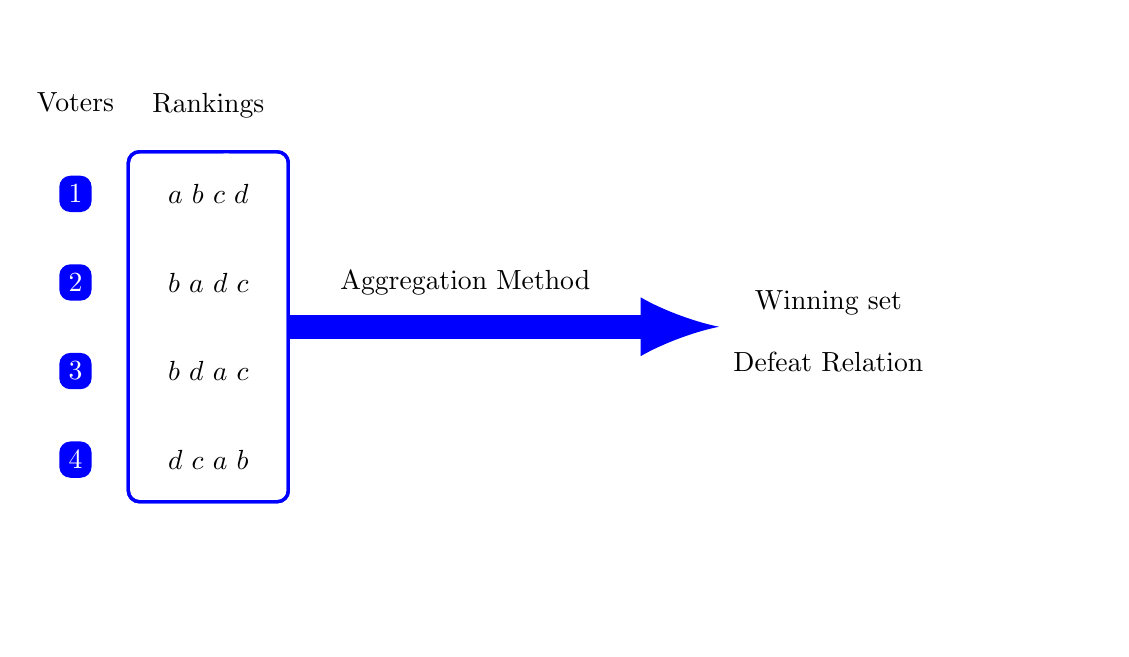
\begin{tikzpicture}[scale=0.75]

\node at (-0.75, 4.55) {Voters}; 

\node[white,rounded corners, fill=blue] at (-0.75,3) {$1$}; 
\node[white,rounded corners,fill=blue] at (-0.75,1.5) {$2$}; 
\node[white,rounded corners,fill=blue] at (-0.75,0) {$3$}; 
\node[white,rounded corners,fill=blue] at (-0.75,-1.5) {$4$}; 

\node[draw=blue,very thick,rounded corners, minimum height=1.75in, minimum width=0.8in] at (1.5,0.75) { };

\node[white]  (pj)  at (5.75, 5.45) {2. Probability judgements}; 

\path[->,draw=white, very thick] (pj) to[out=270, in=90] (1.525, 3.025); 


\node at (1.5, 4.5) {Rankings}; 

\node at (1.5,3) {$a\  b\ c\ d$}; 
\node at (1.5,1.5) {$b\  a\ d\ c$}; 
\node at (1.5,0) {$b\  d\ a\ c$}; 
\node at (1.5,-1.5) {$d\  c\ a\ b$}; 


\node[white]  (prodmod)  at (6, -4) {1. Probabilistically generate preferences}; 

\path[->,draw=white, very thick] (prodmod) to[out=90, in=270] (1.25, -2.25); 



\node[white]  (l)  at (13.75, 3.85) {3. Lottery over candidates}; 

\path[->,draw=white, very thick] (l) to[out=270, in=90] (12, 2.5); 

%\node  at (12, 2.15) {Winner}; 
\node at (12, 1.15) {Winning set}; 
\node  at (12, 0.15) {Defeat Relation}; 
%\node  at (12, -0.85) {Committee}; 
\draw[draw=blue,-latex,line width=3mm] (2.85,0.75) to (10.15,0.75);
 
 \node at (5.85,1.5) {Aggregation Method};
 %   \node[align=center, draw=blue,  fill=blue, text=white, cloud callout, cloud puffs=14, cloud puff arc=90, callout pointer segments=2, anchor=pointer, callout relative pointer={(-120:0.8 cm )}, aspect=4,scale=0.65] at (5.95,1.1) {\begin{minipage}{1.5in}\begin{center}\textcolor{white}{\Large Axiomatic\\Characterization}\end{center}\end{minipage}};
\node[draw=blue,very thick,rounded corners, minimum height=1.75in, minimum width=0.8in] at (1.5,0.75) { };

\end{tikzpicture}

\end{center}
}

\only<2>{
\begin{center}
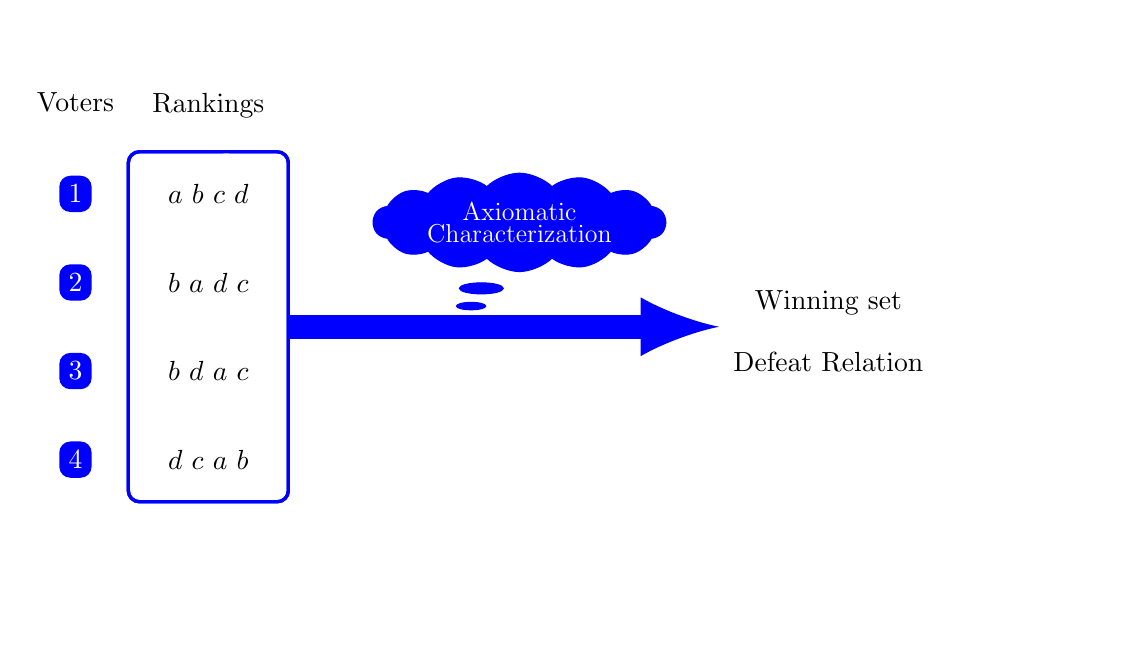
\begin{tikzpicture}[scale=0.75]

\node at (-0.75, 4.55) {Voters}; 

\node[white,rounded corners, fill=blue] at (-0.75,3) {$1$}; 
\node[white,rounded corners,fill=blue] at (-0.75,1.5) {$2$}; 
\node[white,rounded corners,fill=blue] at (-0.75,0) {$3$}; 
\node[white,rounded corners,fill=blue] at (-0.75,-1.5) {$4$}; 

\node[draw=blue,very thick,rounded corners, minimum height=1.75in, minimum width=0.8in] at (1.5,0.75) { };

\node[white]  (pj)  at (5.75, 5.45) {2. Probability judgements}; 

\path[->,draw=white, very thick] (pj) to[out=270, in=90] (1.525, 3.025); 


\node at (1.5, 4.5) {Rankings}; 

\node at (1.5,3) {$a\  b\ c\ d$}; 
\node at (1.5,1.5) {$b\  a\ d\ c$}; 
\node at (1.5,0) {$b\  d\ a\ c$}; 
\node at (1.5,-1.5) {$d\  c\ a\ b$}; 


\node[white]  (prodmod)  at (6, -4) {1. Probabilistically generate preferences}; 

\path[->,draw=white, very thick] (prodmod) to[out=90, in=270] (1.25, -2.25); 



\node[white]  (l)  at (13.75, 3.85) {3. Lottery over candidates}; 

\path[->,draw=white, very thick] (l) to[out=270, in=90] (12, 2.5); 

%\node  at (12, 2.15) {Winner}; 
\node at (12, 1.15) {Winning set}; 
\node  at (12, 0.15) {Defeat Relation}; 
%\node  at (12, -0.85) {Committee}; 
\draw[draw=blue,-latex,line width=3mm] (2.85,0.75) to (10.15,0.75);
 
% \node at (5.85,1.5) {Aggregation Method};
    \node[align=center, draw=blue,  fill=blue, text=white, cloud callout, cloud puffs=14, cloud puff arc=90, callout pointer segments=2, anchor=pointer, callout relative pointer={(-120:0.8 cm )}, aspect=4,scale=0.65] at (5.95,1.1) {\begin{minipage}{1.5in}\begin{center}\textcolor{white}{\Large Axiomatic\\Characterization}\end{center}\end{minipage}};
\node[draw=blue,very thick,rounded corners, minimum height=1.75in, minimum width=0.8in] at (1.5,0.75) { };

\end{tikzpicture}

\end{center}
}




\end{onslide}
\end{frame}


\begin{frame}

\begin{quote}
\textit{social choice theory turns out to be perfectly suitable for mechanical theorem proving...}
\end{quote}
\vfill
\paper{F. Wiedijk}{Arrow's impossibility theorem}{Formalized Mathematics, 15:171–174, 2007}
\vfill

\paper{T. Nipkow}{Social choice theory in HOL: Arrow and Gibbard-Satterthwaite}{Journal of Automated Reasoning, 43:289–304, 2009}
\vfill

\paper{M. Eberl}{Verifying Randomised Social Choice}{International Symposium on Frontiers of Combining Systems, FroCoS 2019: Frontiers of Combining Systems pp 240-256}

\vfill

\paper{F. Brandt, M. Eberl, C. Saile and C. Stricker}{The Incompatibility of Fishburn-Strategyproofness and Pareto-Efficiency}{\url{https://www.isa-afp.org/entries/Fishburn_Impossibility.html}}
\end{frame}

\begin{frame}{Lean}

The Lean Theorem Prover aims to bridge the gap between interactive and automated theorem proving, by situating automated tools and methods in a framework that supports user interaction and the construction of fully specified axiomatic proofs. The goal is to support both mathematical reasoning and reasoning about complex systems, and to verify claims in both domains.


\vfill

\url{https://leanprover.github.io/}
\end{frame}

\begin{frame}


{\Huge Profiles of Preferences}


\end{frame}

\begin{frame}{Profiles}

\begin{definition}\label{ProfileDef} For $V\subseteq\mathcal{V}$ and $X\subseteq\mathcal{X}$, a \emph{$(V,X)$-profile} is a map $\mathbf{P}:V\to \mathcal{B}(X)$. \\[8pt]
Given a $(V,X)$-profile $\mathbf{P}$, let $V(\mathbf{P})$ be $V$ and $X(\mathbf{P})$  be $X$. \\[8pt] We then define a function $\mathsf{Prof}$ that assigns to each pair $(V,X)$ of $V\subseteq\mathcal{V}$ and $X\subseteq\mathcal{X}$ the set $\mathsf{Prof}(V,X)$ of all $(V,X)$-profiles. %Finally, define $\mathsf{PROF} = \bigcup_{V\subseteq\mathcal{V},X\subseteq\mathcal{X}}\mathsf{Prof}(V,X)$.}
\end{definition}


\vfill

%\textnormal{A \textit{profile} is a $(V,X)$-profile for some $V\subseteq\mathcal{V}$ and $X\subseteq\mathcal{X}$.}

%\textnormal{Let $\mathsf{Prof}(V,X)$ be the set of all $(V,X)$-profiles and $\mathsf{Prof}$ the set of all profiles.}

%\whnote{One problem with the above definition is that we cannot extract $X$ from $\mathbf{Q}$, because, e.g., $\mathcal{B}(X)$ may be empty.... In our previous papers, where $\mathbf{Q}(i)$ had to be a linear order, we can extract $X$ from $\mathbf{Q}$---provided there is more than one candidate. If there is only one candidate for $\mathbf{Q}$,  then we cannot extract $X$ from $\mathbf{Q}$....}


\pause
%\begin{itemize}
%\item[] \texttt{def Prof: Type 0 $\to$ Type 0 $\to$ Type 0 := 
%\item[] \qquad\qquad\,\,\, $\lambda$ (V X : Type), V $\to$ X $\to$ X $\to$ Prop}
%\end{itemize}
\begin{itemize}
\item[] \texttt{\textcolor{blue}{def} \textcolor{orange}{Prof} : \textcolor{blue}{Type} $\to$ \textcolor{blue}{Type} $\to$ \textcolor{blue}{Type} := }\\\texttt{$\textcolor{blue}{\lambda}$ (V X : \textcolor{blue}{Type}), V $\to$ X $\to$ X $\to$ \textcolor{blue}{Prop}}
\end{itemize}

\end{frame}

\begin{frame}{Majority Preferred}

\begin{definition}\label{MajPrefDef} \textnormal{Given a profile $\mathbf{P}$ and $x,y\in X(\mathbf{P})$, we say that \textit{$x$ is majority preferred to $y$ in $\mathbf{P}$} if more voters rank $x$ above $y$ than rank $y$ above $x$.}\end{definition}

 \vfill 
 \pause
\begin{itemize}
\item[] \texttt{\textcolor{blue}{def} \textcolor{orange}{majority\_preferred}  $\{$V X : \textcolor{blue}{Type}$\}$ :}

\texttt{Prof V X $\to$ X $\to$ X $\to$ \textcolor{blue}{Prop} := \textcolor{blue}{$\lambda$} P x y,}

\texttt{cardinal.mk $\{$v : V // P v x y$\}$ >\\
cardinal.mk $\{$v : V // P v y x$\}$}
\end{itemize}

\end{frame}

\begin{frame}{Margin}


\begin{definition}\label{MarginDef} \textnormal{Given a profile $\mathbf{P}$ and $x,y\in X(\mathbf{P})$, the \textit{margin of $x$ over $y$ in $\mathbf{P}$}, denoted $Margin_\mathbf{P}(x,y)$, is $|\{i\in V(\mathbf{P})\mid x\mathbf{P}_iy\}|-|\{i\in V(\mathbf{P})\mid y\mathbf{P}_ix\}|$.}
\end{definition}
 
 \vfill 
 \pause
\begin{itemize}
\item[] \texttt{\textcolor{blue}{def} \textcolor{orange}{margin} $\{$V X : \textcolor{blue}{Type}$\}$  [fintype V] : \\ Prof V X $\to$ X $\to$ X $\to$ $\mathbb{Z}$} 

\texttt{:=
    \textcolor{blue}{$\lambda$} P x y, $\uparrow$(finset.univ.filter (\textcolor{blue}{$\lambda$} v, P v x y)).card
        -} \\ \texttt{$\uparrow$(finset.univ.filter (\textcolor{blue}{$\lambda$} v, P v y x)).card}
\end{itemize}

\end{frame}

\begin{frame}

{\Huge Simple Example}

\end{frame}

\begin{frame}{Condorcet Winner and Majority Winner}

\begin{definition}\label{CondorcetDef} \textnormal{Given a profile $\mathbf{P}$ and $x\in X(\mathbf{P})$, $x$ is a \textit{Condorcet winner in $\mathbf{P}$} if for all $y\in X(\mathbf{P})$ with $y\neq x$, $x$ is majority preferred to $y$ in $\mathbf{P}$.\\[8pt] We say that $x$ is a \textit{majority winner in $\mathbf{P}$} if the number of voters who rank $x$ (and only $x$) in first place is greater than the number of voters who do not rank $x$ in first place.}
\end{definition}


\vfill 
\pause 
\begin{itemize}
%\item[] \texttt{\textcolor{blue}{def} \textcolor{orange}{condorcet\_winner} [fintype V] (P : Prof V X) (x : X) :} \\ \texttt{\textcolor{blue}{Prop} := $\forall$ y $\neq$ x, majority\_preferred P x y}
\item[] \texttt{\textcolor{blue}{def} \textcolor{orange}{condorcet\_winner} $\{$V X : \textcolor{blue}{Type}$\}$ (P : Prof V X) (x : X) :} \\ \texttt{Prop := $\forall$ y $\neq$ x, majority\_preferred P x y}
\item[]
%\item[] \texttt{\textcolor{blue}{def} \textcolor{orange}{majority\_winner} [fintype V] (P : Prof V X) (x : X) :} \\ \texttt{\textcolor{blue}{Prop} := (finset.univ.filter ($\lambda$ (v : V), $\forall$ y $\neq$ x, P v x y)).card > (finset.univ.filter ($\lambda$ (v : V), $\exists$ y $\neq$ x, P v y x)).card}
\item[] \texttt{\textcolor{blue}{def} \textcolor{orange}{majority\_winner} $\{$V X : \textcolor{blue}{Type}$\}$ (P : Prof V X) (x : X) :} \\
\texttt{ Prop := cardinal.mk $\{$v : V // $\forall$ y $\neq$ x, P v x y$\}$ > } \\\texttt{ cardinal.mk}  \texttt{$\{$v : V // $\exists$ y $\neq$ x, P v y x$\}$}
\end{itemize}

\end{frame}

\begin{frame}

{\bf Lemma}. For any profile  $\mathbf{P}$, for all $x\in X(P)$, if $x$ is a majority winner in $\mathbf{P}$, then $x$ is a Condorcet winner  in $\mathbf{P}$. 

\vfill 
\begin{itemize}
\item[] \texttt{\textcolor{blue}{lemma} \textcolor{orange}{condorcet\_of\_majority\_winnner} $\{$V X : \textcolor{blue}{Type}$\}$\\ (P : Prof V X)}
\texttt{[fintype V] (x : X) :}

 \texttt{majority\_winner P x $\to$ condorcet\_winner P x :=}

\end{itemize}


\end{frame}


\begin{frame}

We make use of the following theorem from mathlib: 

\bigskip

\begin{itemize}
\item[] \texttt{\textcolor{blue}{theorem} \textcolor{orange}{cardinal.mk\_subtype\_mono} $\{$$\alpha$ : Type u$\}$\\ $\{$$\varphi$ $\psi$ : $\alpha$ $\to$ Prop$\}$} 
\texttt{(h : $\forall$ x, $\varphi$ x $\to$ $\psi$ x) :} \\\texttt{cardinal.mk $\{$x // $\varphi$ x$\}$ $\leq$ cardinal.mk $\{$x // $\psi$ x$\}$}
\end{itemize}
\end{frame}

\begin{frame}
\begin{itemize}
\item[] \texttt{\textcolor{blue}{lemma} \textcolor{orange}{condorcet\_of\_majority\_winnner} $\{$V X : \textcolor{blue}{Type}$\}$\\ (P : Prof V X)}
\texttt{[fintype V] (x : X) :}

 \texttt{majority\_winner P x $\to$ condorcet\_winner P x :=} 

\textcolor{blue}{\texttt{begin}}

\item[\texttt{1.}]\quad  \texttt{intros majority z z\_ne\_x,}  
 
%\item[\texttt{2.}]\quad  \texttt{apply sub\_pos\_of\_lt,}
 
%\item[\texttt{3.}]\quad   \texttt{apply int.coe\_nat\_lt\_coe\_nat\_of\_lt,}

\item[\texttt{2.}]\quad  \texttt{\textcolor{blue}{have} imp1 : $\forall$ v, ($\forall$ y $\neq$ x, P v x y) $\to$ P v x z :=  \\ \quad \textcolor{blue}{by} finish,} 

%\item[\texttt{3.}]\quad\quad  \texttt{$\{$intros v ranks\_x\_first,}

%\item[\texttt{4.}]\quad\quad     \texttt{exact ranks\_x\_first z z\_ne\_x$\}$, }
  
\item[\texttt{3.}]\quad  \texttt{refine lt\_of\_lt\_of\_le \_ (cardinal.mk\_subtype\_mono imp1),} 
 
\item[\texttt{4.}]\quad  \texttt{\textcolor{blue}{have} imp2 : $\forall$ v, P v z x $\to$ ($\exists$ y $\neq$ x, P v y x) :=\\\quad \textcolor{blue}{by} finish,} 
 
% \item[\texttt{7.}]\quad \quad    \texttt{$\{$intros v ranks\_z\_above\_x, }
  
% \item[\texttt{8.}]\quad \quad    \texttt{use [z, z\_ne\_x], }
  
% \item[\texttt{9.}]\quad \quad    \texttt{exact ranks\_z\_above\_x$\}$,}
  
 \item[\texttt{5.}]\quad  \texttt{apply lt\_of\_le\_of\_lt (cardinal.mk\_subtype\_mono imp2),} 
  
\item[\texttt{6.}]\quad  \texttt{exact majority, }
  
\textcolor{blue}{\texttt{end}}
\end{itemize}


\end{frame}

\begin{frame}

{\Huge Functions on Profiles}

\end{frame}
\begin{frame}

\begin{definition} For $V\subseteq\mathcal{V}$ and $X\subseteq\mathcal{X}$, a \textit{social choice correspondence for $(V,X)$}, or $(V,X)$-SCC, is a function  $F: \mathsf{Prof}(V,X)\to \wp(X)$. \\[8pt]


Let $\mathsf{SCC}$ be a function that assigns to each pair $(V,X)$ of $V\subseteq\mathcal{V}$ and $X\subseteq\mathcal{X}$ the set of all $(V,X)$-SCCs.
\end{definition}

\vfill 
\pause 
\begin{itemize}
\item[] \texttt{\textcolor{blue}{def} \textcolor{orange}{SCC} := \textcolor{blue}{$\lambda$} (V X : \textcolor{blue}{Type}), Prof V X $\to$ set X}
\end{itemize}

\vfill 
\pause

\begin{itemize}
%\item[] \texttt{\textcolor{blue}{def} \textcolor{orange}{universal\_domain\_SCC} $\{$V X: \textcolor{blue}{Type}$\}$: SCC V X $\to$ Prop := $\lambda$ F, $\forall$ P, F P $\neq$ $\emptyset$}
\item[] \texttt{\textcolor{blue}{def} \textcolor{orange}{universal\_domain\_SCC} $\{$V X : \textcolor{blue}{Type}$\}$ (F : SCC V X) : Prop :=} \\
\texttt{$\forall$ P : Prof V X, F P $\neq$ $\emptyset$}

\end{itemize}

\end{frame}

\begin{frame}{Example}

The Condorcet SCC: \\[4pt]

\begin{itemize}
\item[] \texttt{\textcolor{blue}{def} \textcolor{orange}{condorcet\_SCC} $\{$V X : \textcolor{blue}{Type}$\}$ : SCC V X := $\textcolor{blue}{\lambda}$ P, }

\texttt{\small $\{$x : X |  condorcet\_winner P x $\vee$  $\neg$ $\exists$ y, condorcet\_winner P y$\}$}
\end{itemize}
\end{frame}

\begin{frame}{Variable-Election Framework}

\begin{definition}\label{VSCC} A \textit{variable-election social choice correspondence} (VSCC) is a function $F$ that assigns to each pair $(V,X)$ of a $V\subseteq \mathcal{V}$ and $X\subseteq\mathcal{X}$ a $(V,X)$-SCC. %We abuse terminology and call the set $\{\mathbf{Q}\in\mathsf{PROF}\mid F(V(\mathbf{Q}),X(\mathbf{Q}))(\mathbf{Q})\neq\emptyset \}$ the \textit{domain} of  $F$. 
%We say that $F$ satisfies  (\textit{finite}) \textit{universal domain} if the domain of $F$ includes $\{\mathbf{P}\in \mathsf{PROF}\mid V(\mathbf{P}) \mbox{ and }X(\mathbf{P}) \mbox{ nonempty and finite}\}$.
\end{definition}


\vfill 

\begin{itemize}
\item[] \texttt{\textcolor{blue}{def} \textcolor{orange}{VSCC} : \textcolor{blue}{Type 1} := $\Pi$ (V X : \textcolor{blue}{Type}), SCC V X}
\end{itemize}

\vfill 
\pause 
Example: Condorcet VSCC\\
\begin{itemize}
\item[] \texttt{\textcolor{blue}{def} \textcolor{orange}{condorcet\_VSCC} : VSCC := \textcolor{blue}{$\lambda$} V X, condorcet\_SCC}
\end{itemize}

\end{frame}

\begin{frame}{Other Functions on Profiles}

\begin{itemize}
\item[] \texttt{\textcolor{blue}{def} \textcolor{orange}{SCC} := \textcolor{blue}{$\lambda$} (V X : \textcolor{blue}{Type}), Prof V X $\to$\colorbox{gray!30}{set X}}
\end{itemize}
\begin{itemize}
\item[] \texttt{\textcolor{blue}{def} \textcolor{orange}{VSCC} : \textcolor{blue}{Type 1} := $\Pi$ (V X : \textcolor{blue}{Type}), SCC V X}
\end{itemize}

\vfill 

\pause 

 \begin{itemize}
\item[] \texttt{\textcolor{blue}{def} \textcolor{orange}{CCR} := \textcolor{blue}{$\lambda$} (V X : \textcolor{blue}{Type}), Prof V X $\to$\colorbox{gray!30}{X $\to$ X $\to$ \textcolor{blue}{Prop}}}
\end{itemize}
\begin{itemize}
\item[] \texttt{\textcolor{blue}{def} \textcolor{orange}{VCCR} := $\Pi$ (V X : \textcolor{blue}{Type}), CCR V X}
\end{itemize}


\vfill 
\pause 


Given an asymmetric VCCR $f$, we define the \textit{maximal-element induced} VSCC $f_{M}$: 

\begin{itemize}
\item[] \texttt{\textcolor{blue}{def} \textcolor{orange}{max\_el\_VSCC} : VCCR $\to$ VSCC := \textcolor{blue}{$\lambda$} f V X P,} \\
\texttt{$\{$x : X | $\forall$ y : X, $\neg$ f V X P y x$\}$}
\end{itemize}

\end{frame}
\begin{frame}{Formalized Proofs}

 
We verified  all the results about a new voting method, {\em Split Cycle}, from

\bigskip

\paper{W. Holliday and E. Pacuit}{Split Cycle: A New Condorcet Consistent Voting Method Independent of Clones and Immune to Spoilers
}{\url{https://arxiv.org/abs/2004.02350}}
 \end{frame}
 
 \begin{frame}
 
 \renewcommand{\arraystretch}{1.3}

\begin{center}{\small \begin{tabular}{l|c|c|c|c|c|c|c|}
 &  \makecell{  Split\\[-2pt] Cycle}  &  \makecell{\textcolor{gray!60}{Ranked}\\[-2pt] \textcolor{gray!50}{Pairs}} & \makecell{\textcolor{gray!60}{Beat}\\[-2pt]\textcolor{gray!60}{Path}} & \makecell{\textcolor{gray!60}{Mini-}\\[-2pt]\textcolor{gray!60}{max}}  &   \makecell{\textcolor{gray!60}{GETCHA/}\\[-2pt]\textcolor{gray!60}{GOCHA}}    &   \makecell{\textcolor{gray!60}{Ranked}\\[-2pt] \textcolor{gray!60}{Choice}} &  \textcolor{gray!60}{Plurality}\\\Xhline{3\arrayrulewidth}
 
{Condorcet Winner} & \cellcolor{gray!50}{$\checkmark$} & \cellcolor{gray!50}{$\checkmark$} & \cellcolor{gray!50}{$\checkmark$} & \cellcolor{gray!50}{$\checkmark$} & \cellcolor{gray!50}{$\checkmark$} & \cellcolor{gray!50}{$-$} &  \cellcolor{gray!50}{$-$} \\\hline

{Condorcet Loser} & \cellcolor{white}{$\checkmark$} & \cellcolor{white}{$\checkmark$}& \cellcolor{white}{$\checkmark$}& \cellcolor{white}{$-$} & \cellcolor{white}{$\checkmark$}& \cellcolor{white}{$\checkmark$} &  \cellcolor{white}{$-$} \\\hline

{Pareto} & \cellcolor{gray!50}{$\checkmark$} & \cellcolor{gray!50}{$\checkmark$}&\cellcolor{gray!50}{$\checkmark$} &\cellcolor{gray!50}{$\checkmark$} & \cellcolor{gray!50}{$-$} & \cellcolor{gray!50}{$\checkmark$} & \cellcolor{gray!50}$\checkmark$\\\hline

{Monotonicity} & \cellcolor{white}{$\checkmark$} & \cellcolor{white}{$\checkmark$}&\cellcolor{white}{$\checkmark$} &\cellcolor{white}{$\checkmark$} & \cellcolor{white}{$\checkmark$} & \cellcolor{white}{$-$} & \cellcolor{white}$\checkmark$\\\hline

\makecell[l]{{Independence of}\\[-2pt] {Clones}} & \cellcolor{gray!50}$\checkmark$&\cellcolor{gray!50}$\checkmark$ &\cellcolor{gray!50}$\checkmark$ &\cellcolor{gray!50}$-$ &\cellcolor{gray!50}$\checkmark$ &\cellcolor{gray!50}$\checkmark$&\cellcolor{gray!50}$-$ \\\hline

% \makecell[l]{ {Immunity to}\\[-2pt] {Spoilers}} & \cellcolor{white}$\checkmark$&\cellcolor{white}$-$ & \cellcolor{white}$-$& \cellcolor{white}$\checkmark$& \cellcolor{white}{$\checkmark$} & \cellcolor{white}$-$ &\cellcolor{white}$-$ \\\hline
 
  \makecell[l]{ Strong {Stability for}\\[-2pt] {Winners}} & \cellcolor{white}$\checkmark$&\cellcolor{white}$-$ & \cellcolor{white}$-$& \cellcolor{white}$-$& \cellcolor{white}{$\checkmark$} & \cellcolor{white}$-$ &\cellcolor{white}$-$ \\\hline
  
 %\makecell[l]{{Amalgamation}} & \cellcolor{white}$\checkmark$&\cellcolor{white}$-$ & \cellcolor{white}$-$& \cellcolor{white}$-$& \cellcolor{white}{$\checkmark$/$-$} & \cellcolor{white}$-$ &\cellcolor{white}$-$ \\\hline
%{Rejectability} & \cellcolor{gray!50}$\checkmark$& \cellcolor{gray!50}$\checkmark$& \cellcolor{gray!50}$\checkmark$ & \cellcolor{gray!50}$\checkmark$& \cellcolor{gray!50}$-$ & \cellcolor{gray!50}$\checkmark$ & \cellcolor{gray!50}$\checkmark$\\\Xhline{3\arrayrulewidth}

%\makecell[l]{{Smith}} & \cellcolor{white}$\checkmark$&\cellcolor{white}$\checkmark$& \cellcolor{white}$\checkmark$&\cellcolor{white}$-$ & \cellcolor{white}$\checkmark$&\cellcolor{white}$-$ &\cellcolor{white}$-$ \\\hline

%\makecell[l]{{ISDA}} & \cellcolor{gray!50}$\checkmark$&\cellcolor{gray!50}$\checkmark$& \cellcolor{gray!50}$\checkmark$&\cellcolor{gray!50}$-$ & \cellcolor{gray!50}$\checkmark$&\cellcolor{gray!50}$-$ &\cellcolor{gray!50}$-$ \\\hline

%\makecell[l]{Resolvability} & $-$& $\checkmark$& $\checkmark$ & $\checkmark$& $-$ & $\checkmark$ & $\checkmark$\\\hline
\makecell[l]{{Reversal Symmetry}} & \cellcolor{gray!50}$\checkmark$&\cellcolor{gray!50}$\checkmark$& \cellcolor{gray!50}$\checkmark$&\cellcolor{gray!50}$-$ & \cellcolor{gray!50}$\checkmark$&\cellcolor{gray!50}$-$ &\cellcolor{gray!50}$-$ \\\hline

\makecell[l]{{Positive Involvement}} & \cellcolor{white}$\checkmark$&\cellcolor{white}$-$& \cellcolor{white}$-$&\cellcolor{white}$\checkmark$ & \cellcolor{white}$\checkmark$/$-$ &\cellcolor{white}$\checkmark$ &\cellcolor{white}$\checkmark$ \\\hline

\makecell[l]{{Negative Involvement}} & \cellcolor{gray!50}$\checkmark$&\cellcolor{gray!50}$-$& \cellcolor{gray!50}$-$&\cellcolor{gray!50}$\checkmark$ & \cellcolor{gray!50}$\checkmark$/$-$&\cellcolor{gray!50}$-$ &\cellcolor{gray!50}$\checkmark$ \\\hline

\end{tabular}}
\end{center}

 \end{frame}
 
 \begin{frame}{Future Work}
 
 \begin{itemize}
 %\item Results about Split Cycle do not depend on properties of the voters' preferences.
 %\vfill
 %\item Can we generalize the definition of margin? E.g.,  $(a,b)\succ_\mathbf{P} (c,d)$ means that the strength of majority preference for $a$ over $b$ in profile $\mathbf{P}$ is {\em stronger} than the strength of majority preference for $c$ over $d$ in $\mathbf{P}$.
 %\vfill
 \item Verify axioms of other voting methods: Not just margin-based methods (e.g., Split Cycle and Beat Path), but also  scoring rules (e.g., Plurality and Borda), and {\em recursive} voting methods (e.g., Instant Runoff).
 \vfill
 \item Formalize characterization theorems (e.g., Arrow's Theorem characterizing dictatorship, May's Theorem characterizing majority rule, Young's Theorem characterizing scoring rules, $\ldots$).
 \vfill
 \end{itemize}
 
 
 \end{frame}
 
 \begin{frame}
 
 \begin{center}{\Large Thank you!}\\[4pt]
 \url{https://github.com/chasenorman/Formalized-Voting}
 \end{center}
 \end{frame}
\end{document}